\section{Results} \label{section: results}
The airflow $Q$ through a cross-sectional area $A$ can be mathematically defined as:
\begin{gather}
    Q = \int_A \rho \mathbf{v} \cdot d\mathbf{A} = \frac{dm}{dt} \label{eq: flow_rate}
\end{gather}
The airflow $Q$ was periodically calculated and stored over the duration of the simulation.

\begin{figure}[H]
    \centering
    \begin{subfigure}[b]{0.47\textwidth}
        \centering
        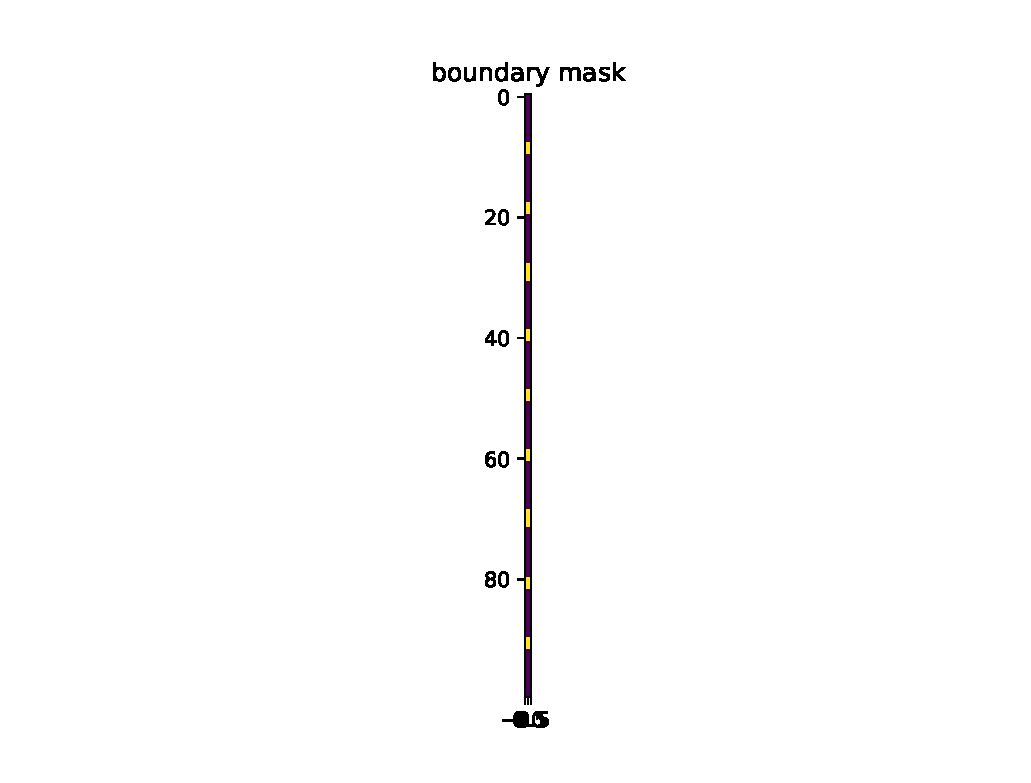
\includegraphics[width=\textwidth]{figures/bound_ex3.pdf}
        \caption{Example of a boundary mask representing a window with a bug grid.}
        \label{fig: bound1}
    \end{subfigure}
    \hfill
    \begin{subfigure}[b]{0.47\textwidth}
        \centering
        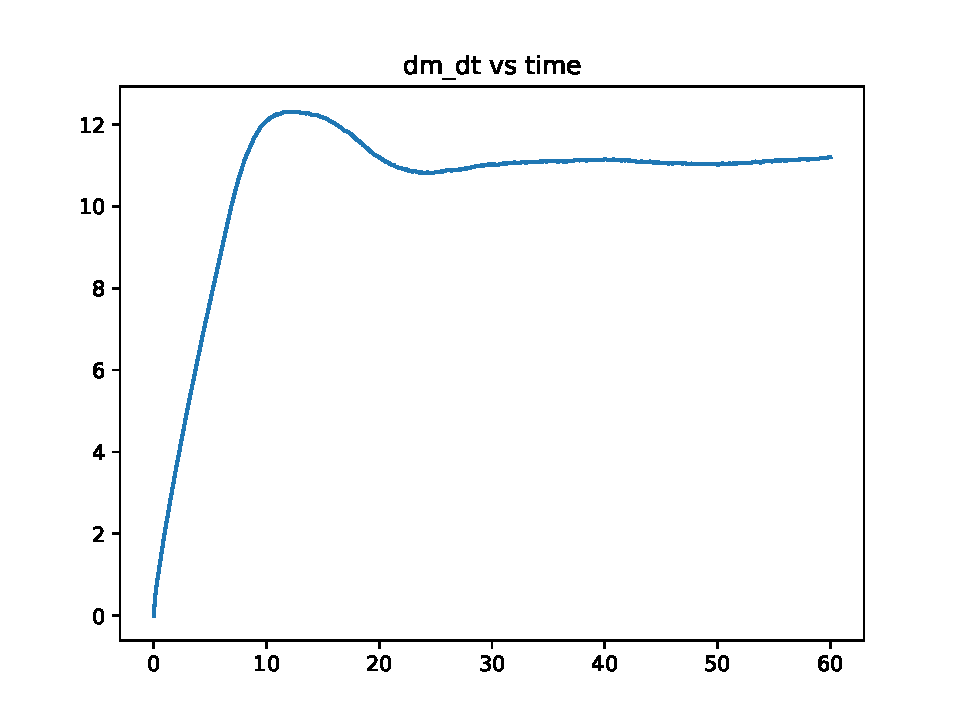
\includegraphics[width=\textwidth]{figures/dm_dt/log_holecount_10_holewidth_0.4_repeat_1.pdf}  % 10, 0.4
        \caption{The plot of airflow $Q$ against time, hole count = 10, hole width = 0.4.}
        \label{fig: flowrate1}
    \end{subfigure}
    \caption{Comparison of airflow rates through the cross-sectional area of the window for different grid hole sizes.}
    \label{fig: bound_plos_flowrate1}
\end{figure}

\begin{figure}[H]
    \centering
    \begin{subfigure}[b]{0.47\textwidth}
        \centering
        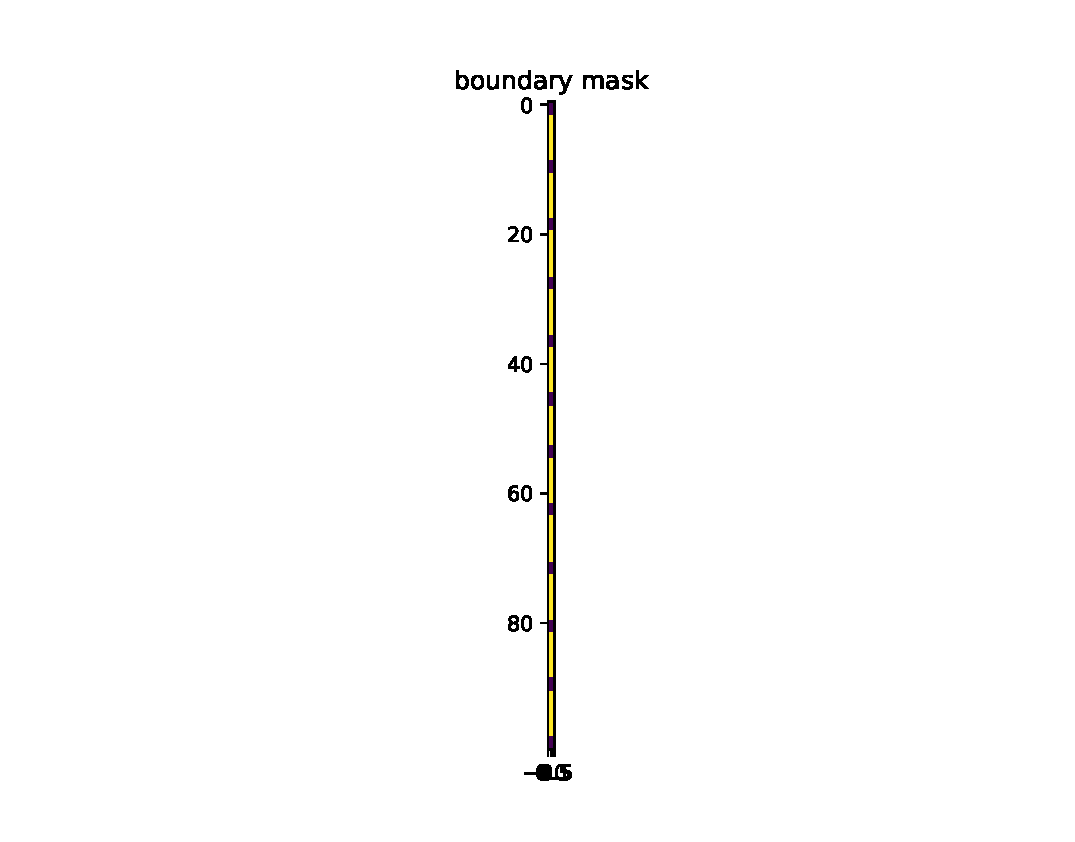
\includegraphics[width=\textwidth]{figures/bound_ex2.pdf}
        \caption{Example of a boundary mask representing a window with a bug grid.}
        \label{fig: bound2}
    \end{subfigure}
    \hfill
    \begin{subfigure}[b]{0.47\textwidth}
        \centering
        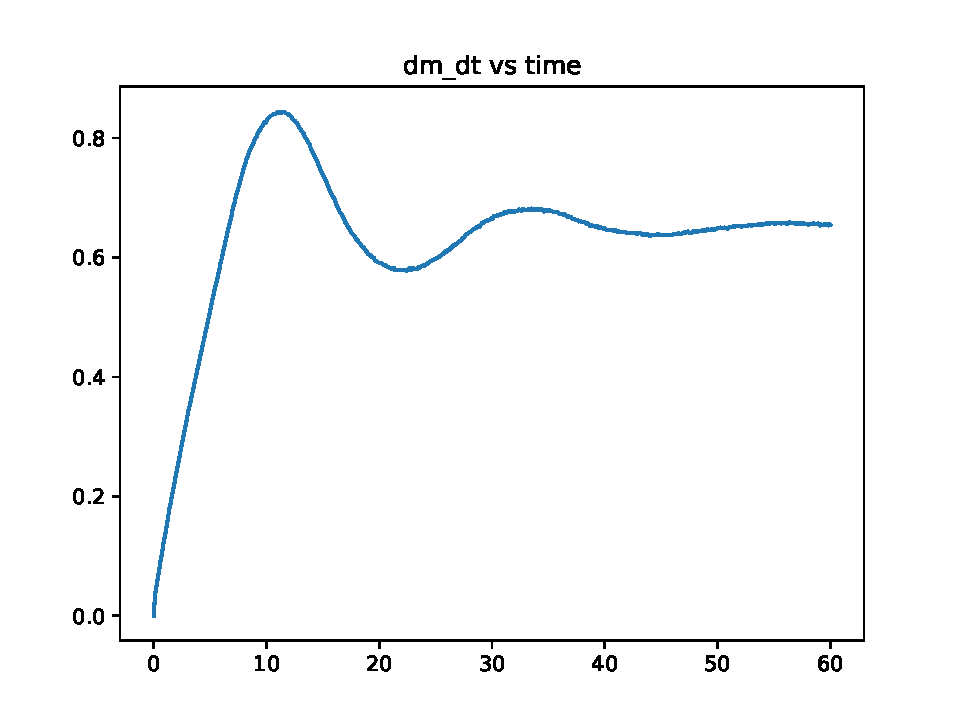
\includegraphics[width=\textwidth]{figures/dm_dt/log_holecount_12_holewidth_0.1_repeat_1.pdf}  % 12, 0.1
        \caption{The plot of airflow $Q$ against time, hole count = 12, hole width = 0.1.}
        \label{fig: flowrate2}
    \end{subfigure}
    \caption{Comparison of airflow rates through the cross-sectional area of the window for different grid hole sizes.}
    \label{fig: bound_plos_flowrate2}
\end{figure}

\begin{figure}[H]
    \centering
    \begin{subfigure}[b]{0.47\textwidth}
        \centering
        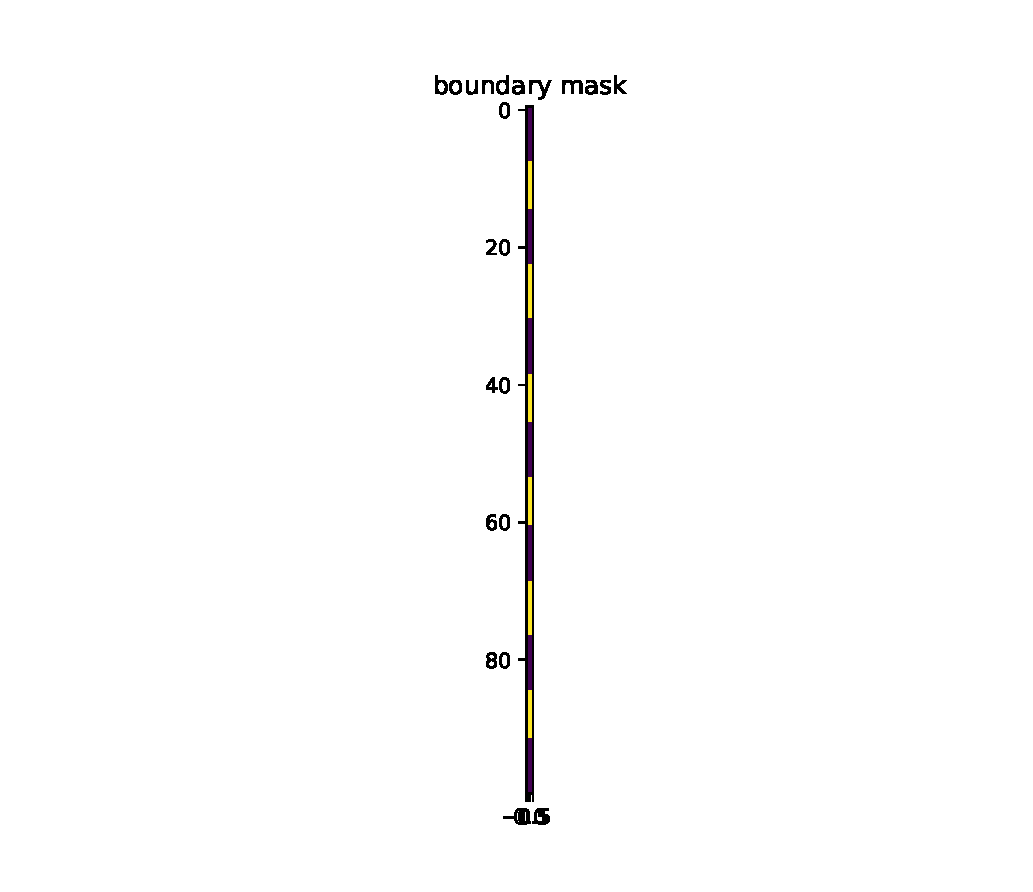
\includegraphics[width=\textwidth]{figures/bound_ex1.pdf}
        \caption{Example of a boundary mask representing a window with a bug grid.}
        \label{fig: bound3}
    \end{subfigure}
    \hfill
    \begin{subfigure}[b]{0.47\textwidth}
        \centering
        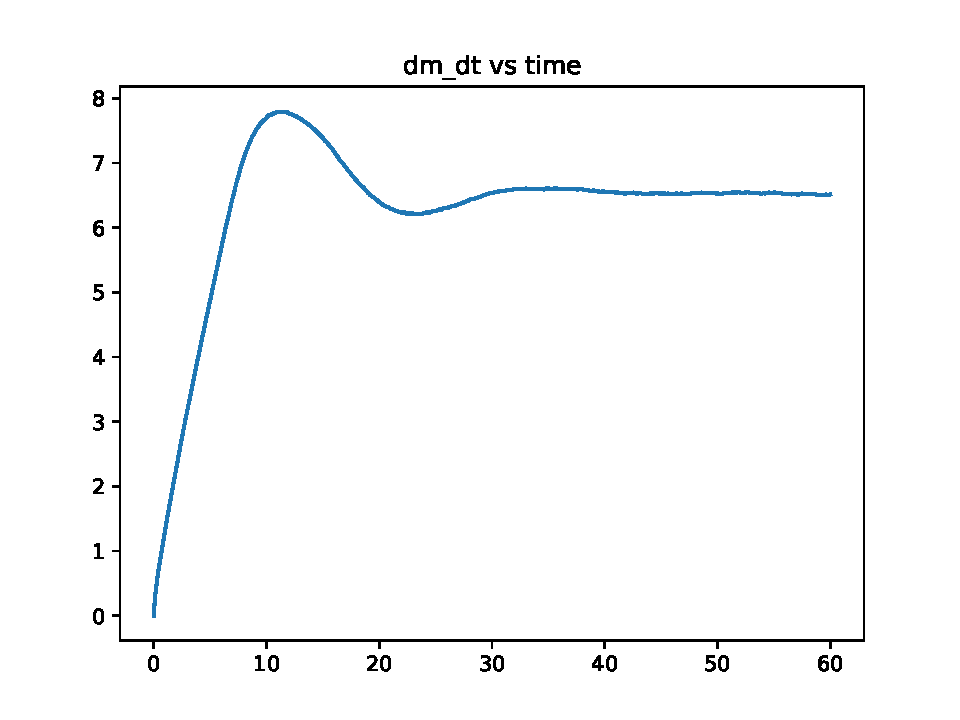
\includegraphics[width=\textwidth]{figures/dm_dt/log_holecount_7_holewidth_0.4_repeat_1.pdf}  % 7, 0.4
        \caption{The plot of airflow $Q$ against time, hole count = 7, hole width = 0.4.}
        \label{fig: flowrate3}
    \end{subfigure}
    \caption{Comparison of airflow rates through the cross-sectional area of the window for different grid hole sizes.}
    \label{fig: bound_plos_flowrate3}
\end{figure}

% TODO: Add some of the field plots here as well + discuss later


From Eq. (\ref{eq: flow_rate}), the total mass $m$ of air that flows through the area in time $T$ is given by:
\begin{gather}
    m = \int_0^T Q ~dt
\end{gather}

 The plot of $m$ against the number of holes in the grid was plotted in Figure \ref{fig: flow_rate} for four different hole sizes.
\begin{figure}[H]
    \centering
    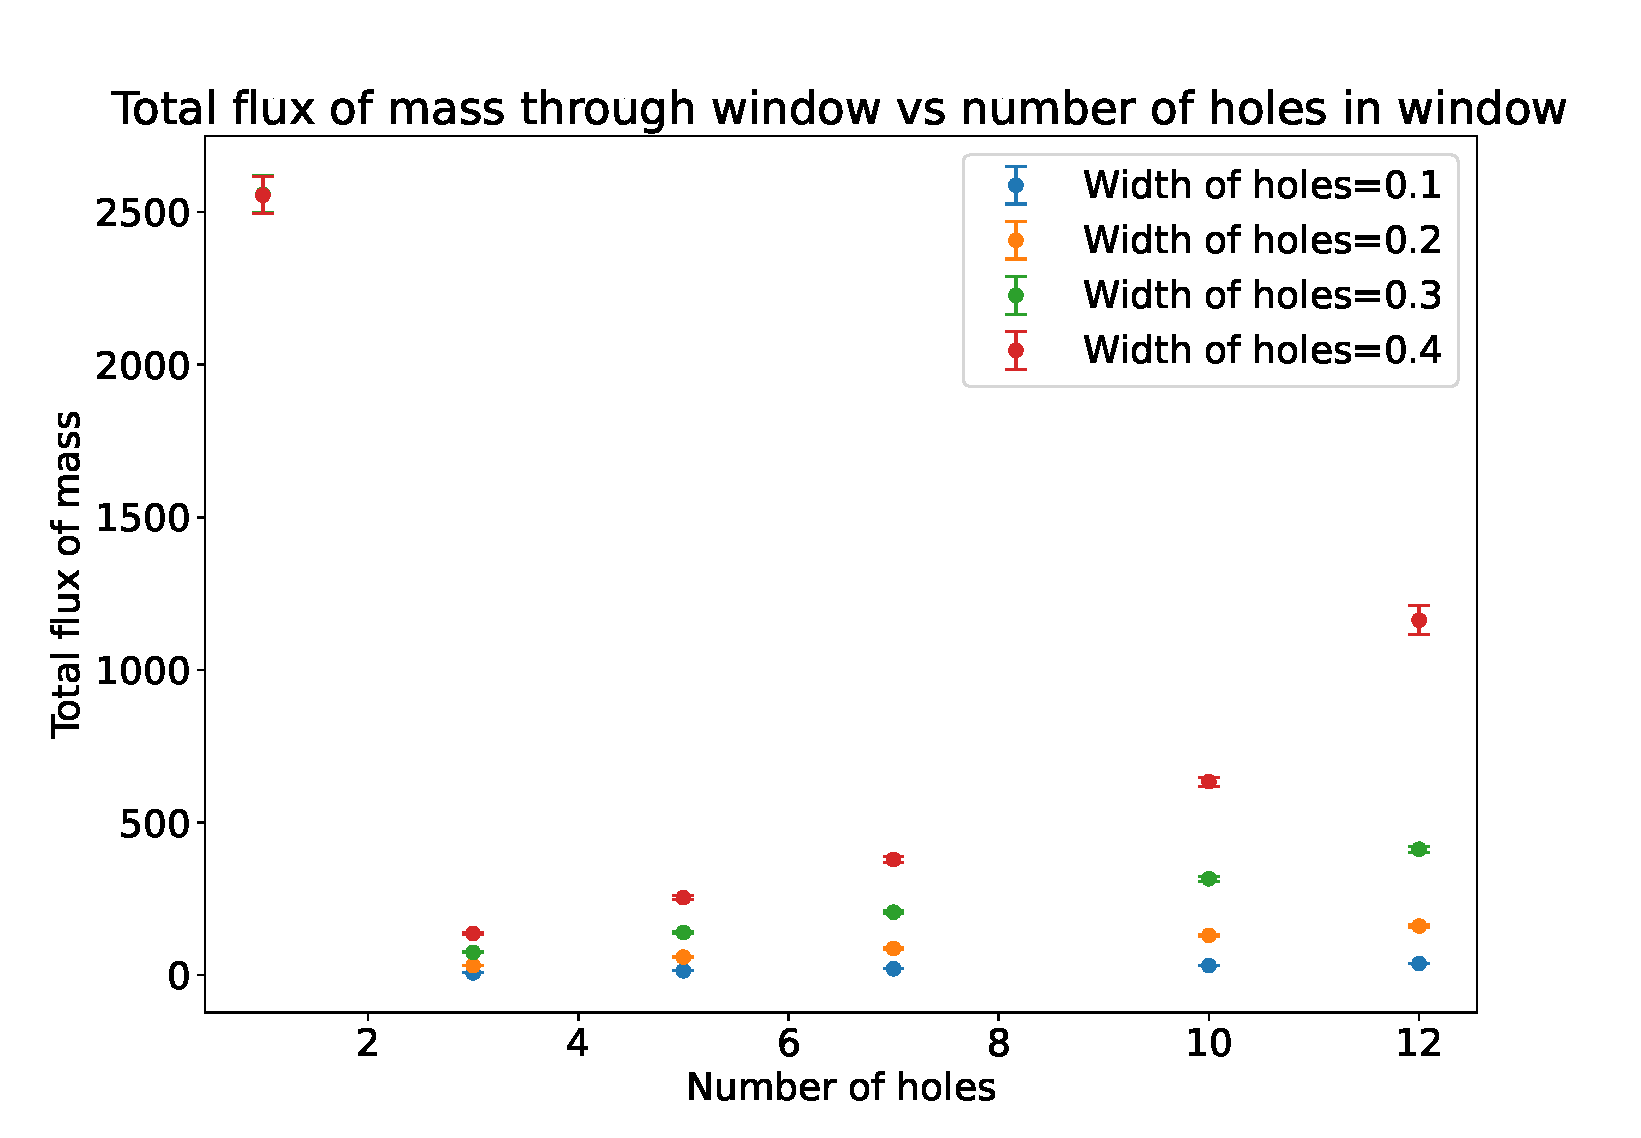
\includegraphics[width=0.8\textwidth]{figures/flux_vs_holes.pdf}
    \caption{Total mass $m$ through the cross-sectional area of the window vs. the number of holes in the bug grid, plotted for different grid hole sizes.}
    \label{fig: flow_rate}
\end{figure}
In the left-upper corner of Figure \ref{fig: flow_rate}, the data point corresponding to an empty window is present. Note that this value was constantly the same for all widths of the hole, regardless of its colour in the plot. We can also see, that the airflow through the window increases both with the number of holes and the size of the holes. \\

\begin{figure}[H]
    \centering
    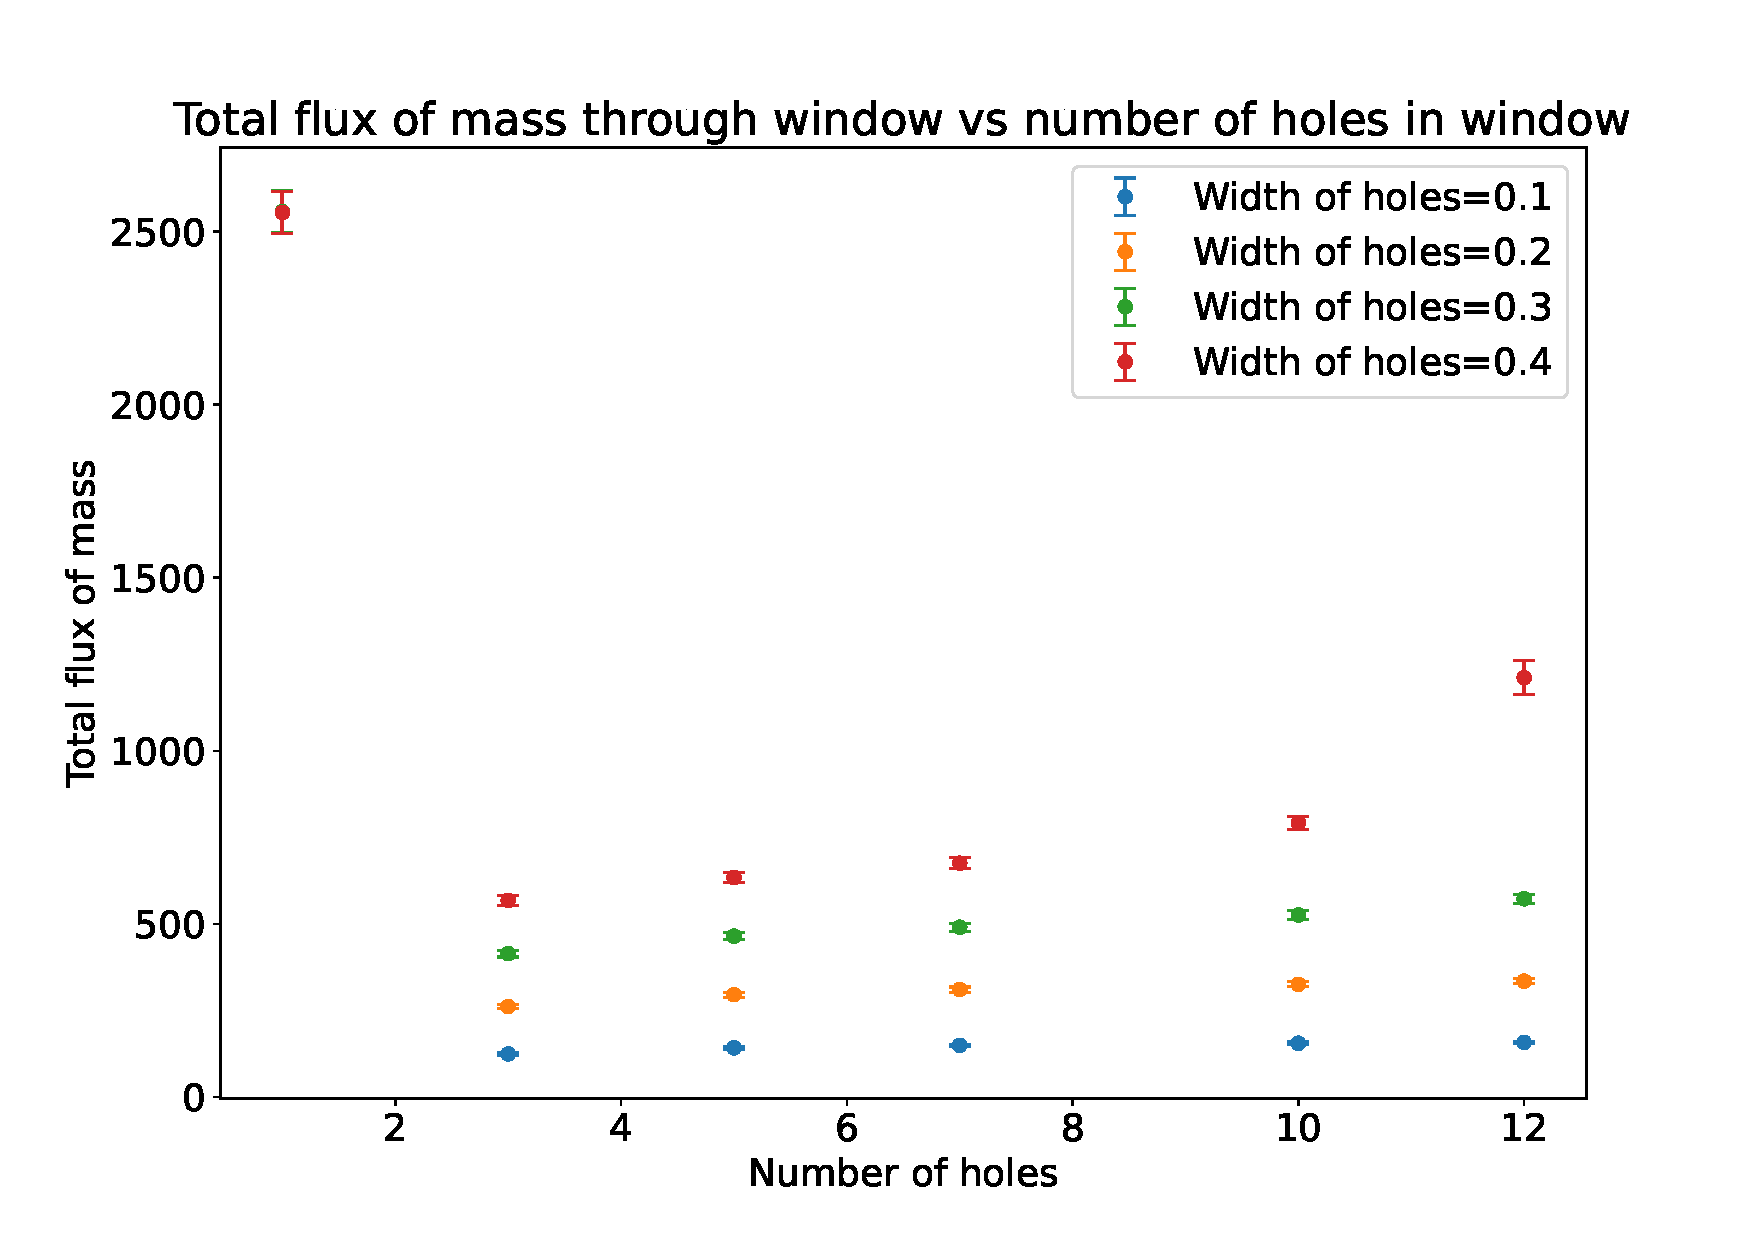
\includegraphics[width=0.8\textwidth]{figures/flux_vs_holes_norm.pdf}
    \caption{Normalized total mass $m$ through the cross-sectional area of the window vs. the number of holes in the bug grid, plotted for different grid hole sizes.}
    \label{fig: flow_rate_norm}
\end{figure}
Figure \ref{fig: flow_rate_norm} displays the same data as Figure \ref{fig: flow_rate}, but the airflow is normalized to the actual effective area of the window. We can see that the normalized airflow still increases with the size of the holes, however, the number of holes no longer has a significant impact.


